\documentclass{article}

% NeurIPS 2024 style (preprint mode via [final], matching the GAUSE companion)
\usepackage[final]{neurips_2024}

\usepackage[utf8]{inputenc}
\usepackage[T1]{fontenc}
\usepackage{lmodern}
\usepackage{hyperref}
\usepackage{url}
\usepackage{booktabs}
\usepackage{amsfonts}
\usepackage{amsmath}
\usepackage{amssymb}
\usepackage{nicefrac}
\usepackage{microtype}
\usepackage{graphicx}
\usepackage{algorithm}
\usepackage{algorithmic}
\usepackage{xcolor}
\usepackage{multirow}
\usepackage{subcaption}
\usepackage{amsthm}
\usepackage{colortbl}

% Theorem environments
\newtheorem{proposition}{Proposition}
\newtheorem{lemma}{Lemma}
\newtheorem{definition}{Definition}
\newtheorem{remark}{Remark}
\newtheorem{assumption}{Assumption}
\newtheorem{observation}{Observation}

% Custom commands
\newcommand{\R}{\mathbb{R}}
\newcommand{\E}{\mathbb{E}}
\newcommand{\Var}{\mathrm{Var}}
\newcommand{\TV}{\mathrm{TV}}
\newcommand{\KL}{\mathrm{KL}}
\newcommand{\nm}{\textsc{RISP}}
\newcommand{\regret}{\rho}
\newcommand{\Ginv}{G_{\mathrm{inv}}}
\newcommand{\Gforget}{G_{\mathrm{forget}}}
\DeclareMathOperator*{\argmax}{arg\,max}
\DeclareMathOperator*{\argmin}{arg\,min}

\title{When the Regime Returns:\\
Retention and Invariance in Decision-Focused Strategy Pools\\
for Non-Stationary Markets}

\author{
  Yuhao Li\\
  University of Pennsylvania \\
  \texttt{li88@sas.upenn.edu}
}

\begin{document}

\maketitle

\begin{abstract}
Financial markets are non-stationary in two distinct ways that existing
strategy-allocation methods conflate. \textbf{Between regimes}, market states
(trend, range, high-volatility, crisis) switch and recur on irregular
schedules with long dormancy, so a reward-chasing capital allocator---recent-P\&L
weighting or a learned mixture-of-experts router---starves and overwrites the
dormant-regime specialist and pays a full recalibration cost exactly when the
regime returns. \textbf{Within a regime}, each recurrence is a different draw
from the regime's environment distribution (the 2008 crisis is not 2020 is not
2022), so a specialist trained by empirical risk minimization on past episodes
of its own regime still fails out-of-distribution on the next one. We show
these failure modes are governed by \emph{independent} design choices and
propose \nm{} (Regime-Invariant Specialist Pools), a pool of capacity-bounded,
decision-focused specialists in which (i)~regimes are acquired by batched
winner-take-all competition, yielding a converged regime-to-specialist
assignment that is \emph{independent of current reward}---the crisis
specialist idles through calm markets and retains its calibration by identity,
not P\&L---and (ii)~each specialist trains its niche with a decision-focused
\emph{invariance} objective (variance plus mean of an SPO-style regret
surrogate across historical episodes of its regime). We prove a
post-reactivation regret bound that decomposes into a \emph{forgetting
deficit}---zero for any reward-independent assignment, approaching the full
relearning cost for any reward-driven one---and an \emph{invariance gap}
controlled by the episode-variance penalty, including the
Pinsker-type bridge from divergence-metric invariance to regret. In controlled
regime-switching markets with realistic signal-to-noise, the predicted
$2{\times}2$ dissociation holds with all pre-registered orderings confirmed
(20 seeds, Holm-corrected): emergent reward-independent assignment cuts
post-reactivation decision regret by $6.1\%$ versus a capacity-matched
monolith ($p{=}1.3{\times}10^{-3}$), the invariance objective cuts it a
further $4.4\%$ ($p{=}6.1{\times}10^{-3}$; $10.3\%$ jointly,
$p{=}9.2{\times}10^{-7}$; $38\%$ of the excess over the irreducible noise
floor), and the interaction is \emph{super-additive}: invariant training buys
nothing in a reward-driven monolith ($p{=}0.88$ vs.\ ERM), because an objective
cannot help a head that has been evicted. The learned router and the
recent-performance allocator inherit the monolith's failure; the full system
is statistically indistinguishable from a hand-pinned oracle assignment
trained with the same objective ($p{=}0.72$)---recovering the skyline without
being handed the assignment---and nominally beats the oracle assignment
trained with ERM. We pair the
mechanism with an honest audit in the GAUSE tradition: a pre-registered
structure diagnostic run on real crypto and commodity panels finds \emph{no
exploitable regime structure on the decision-regret metric} under causal,
leakage-free labelings---so the real-data $2{\times}2$ is correctly null, the
mechanism's preconditions are checkable before deployment, and we quantify
exactly when retention is worthless (high signal-to-noise relearning,
short dormancy, structureless regimes). All claims are regret and retention
claims, not alpha claims; code, data, and per-figure result files are
released.
\end{abstract}

%=============================================================================
\section{Introduction}
%=============================================================================

A multi-strategy fund maintains playbooks for market conditions that are
mostly absent: the crisis desk idles through years of calm; the
short-volatility book hibernates through stress. The allocation question that
governs such a system---\emph{which strategy gets capital, attention, and
recalibration today, and who keeps a strategy whose regime is dormant?}---has
a standard machine-learning answer (route by recent reward: a learned gate, a
recent-Sharpe weighting) and a standard failure mode that the GAUSE companion
study isolated in controlled prediction domains \citep{li2026gause}: a dormant
regime emits no reward, so any allocator that protects capacity using current
reward is structurally blind to exactly the knowledge that most needs
protection. When the regime returns, the system relearns what it once knew,
and in markets the relearning window---the first days of a crisis---is
precisely when decisions are most consequential.

This paper develops that observation into a theory and system for
\emph{decision-focused} learning in non-stationary markets, and in doing so
isolates a second, orthogonal failure mode that the retention story alone
misses. Suppose the crisis specialist \emph{is} protected---its parameters
untouched through dormancy. Protection guarantees only that the specialist
still knows \emph{the last crisis}. Each occurrence of a regime is a distinct
draw from that regime's environment distribution: flight-to-quality
correlations, volatility clustering, and liquidity spirals recur
\emph{structurally}, but the surface features that carried them in 2008
differ from 2020 and from 2022. A specialist trained by empirical risk
minimization (ERM) on its own regime's history loads on episode-specific
("spurious") regularities and fails out-of-distribution on the next episode
\citep{arjovsky2019irm, yan2026invpnco}. Retention solves \emph{between-regime}
forgetting; it does nothing for \emph{within-regime} drift.

Our central claim is that these are \textbf{two orthogonal kinds of
non-stationarity}, addressed by \emph{independent} mechanisms:

\begin{itemize}
    \item \textbf{(N1) Between-regime switching} is an \emph{allocation}
    problem. It is solved by any capacity assignment that is
    \emph{independent of current reward} and persistently covers the regime
    inventory---so that the dormant specialist receives no foreign updates and
    retains by identity. No training objective can substitute: a forgotten
    head is gone regardless of the loss it was trained with.
    \item \textbf{(N2) Within-regime drift} is a \emph{training-objective}
    problem. It is solved by an invariance objective across the regime's
    historical episodes---penalizing the variance of a decision-focused
    (SPO-style) regret surrogate across episodes so the specialist learns the
    decision-relevant structure common to \emph{all} crises rather than the
    idiosyncrasies of the last one. No allocation mechanism can substitute:
    retention of an episode-overfit head retains the overfitting too.
\end{itemize}

The paper's single falsifiable claim is the resulting $2{\times}2$:
crossing allocation mechanism (reward-driven vs.\ reward-independent) with
training objective (ERM vs.\ invariant) should produce monotone improvement
along both axes in post-reactivation decision regret, with a signature
asymmetry---the invariance axis should be inert in the reward-driven row,
because an evicted head cannot benefit from the objective that trained it.
Our experiments confirm every cell of this prediction, including the
asymmetry (Section~\ref{sec:e1}), and our theory derives it
(Section~\ref{sec:theory}).

\paragraph{Scope statement (the sleeping-experts deflation, addressed up
front).} The contribution concerns capacity-bounded \emph{learners}, not
combinations of fixed experts. Sleeping-experts and adaptive-regret schemes
\citep{freund1997sleeping, hazan2009adaptive, daniely2015strongly} also
freeze dormant experts' state---but only because their experts are
\emph{static strategies} with nothing to forget. The problem \nm{} solves
arises precisely when specialists must keep \emph{learning} within their
niche under bounded capacity, so that reward-driven reallocation causes
destructive interference across regimes. We operationalize this distinction
as a baseline pair: Hedge over \emph{fixed} strategies retains trivially but
cannot adapt within-regime and is dominated by every learning arm
(Section~\ref{sec:e1}); Hedge over capacity-bounded \emph{learning} experts
inherits the interference failure and tracks the monolith. The most dangerous
related work thus becomes a supporting experiment.

\paragraph{Contributions.}
\begin{enumerate}
    \item \textbf{Problem decomposition (C1).} We formally decompose
    non-stationary financial decision error into a between-regime
    \emph{forgetting deficit} and a within-regime \emph{invariance gap}, and
    show---in theory and experiment---that they are governed by independent
    design choices (allocation vs.\ training objective), with a predicted and
    confirmed super-additive interaction: invariant training pays \emph{only}
    inside a retaining allocation.
    \item \textbf{Method (C2).} \nm{}: the first strategy-pool architecture
    combining reward-independent, emergent (competition-driven) capacity
    assignment with decision-focused invariant learning per niche. The
    anticipated financial adaptation of the GAUSE competition mechanism is a
    \emph{batched} winner-take-all window ($W_c$ days of cumulative
    within-regime regret); we pre-registered the expectation that per-step
    competition would converge to noise at realistic signal-to-noise, and
    report honestly that the expectation is \emph{not} borne out---the
    exponentiated-gradient affinity accumulation across windows performs the
    necessary averaging, and the mechanism is robust across
    $W_c \in \{1, \dots, 60\}$ (Section~\ref{sec:e5}). No gate is trained,
    no freezing schedule is set, no regime-to-desk map is designed.
    \item \textbf{Theory (C3).} A post-reactivation regret bound
    $\E[\regret_{\mathrm{react}}] \le \Ginv + \Gforget$
    (Proposition~\ref{prop:decomp}) in which $\Gforget = 0$ for \emph{any}
    reward-independent covering assignment while reward-driven assignment
    drives it to the full relearning cost at an explicit rate
    (Proposition~\ref{prop:dichotomy}); $\Ginv$ is controlled by the
    episode-variance penalty (Lemma~\ref{lem:transfer}), with an explicit
    Pinsker-type bridge from divergence-metric invariance statements to the
    regret metric (Lemma~\ref{lem:bridge})---closing the technical gap
    between Inv-PnCO-style guarantees \citep{yan2026invpnco} and decision
    regret. A break-even analysis (Proposition~\ref{prop:breakeven}) gives
    the dormancy window in which retention pays once idle-specialist carrying
    costs are charged.
    \item \textbf{Evaluation protocol (C4).} A diagnostic-first standard for
    regime-aware financial ML: \emph{post-reactivation regret} in a probe
    window after each reactivation, leakage-free causal regime labelings, and
    a pre-registered structure diagnostic run \emph{before} claiming gains.
    On our real panels (crypto, commodities) the diagnostic correctly
    \emph{fails}---no exploitable regime structure on the decision metric
    under causal labels---and the real-data dissociation is, as the
    methodology then requires, null. We report this prominently rather than
    burying it: where the diagnostic fails, no regime-aware mechanism (ours
    included) can be bought, and a method that had claimed otherwise would be
    fitting noise.
    \item \textbf{Honest audit (C5).} Conditions under which \nm{} does
    \emph{not} pay, each quantified: slack capacity ($K \to R$ closes the
    monolith gap); high within-regime signal-to-noise (a fresh learner
    recalibrates within days, making retention worthless---we sweep the
    break-even relearning speed); short dormancy (the retention gap grows
    with dormancy length); structureless regimes (the E0 gate); and carrying
    costs above the break-even threshold.
\end{enumerate}

We emphasize register throughout: our claims are \emph{regret and retention}
claims about a mechanism, demonstrated where its preconditions verifiably
hold, not alpha claims about live markets. The honest result on present real
data is that the preconditions do \emph{not} hold there at daily frequency
under our labelers and feature inventory---a finding the diagnostic-first
protocol is designed to surface, and one consistent with the GAUSE oracle
audit on the prediction metric \citep{li2026gause}.

%=============================================================================
\section{Related Work}
%=============================================================================

\paragraph{Regime-switching finance.} Markov-switching models
\citep{hamilton1989new}, regime effects in asset returns
\citep{ang2012regime}, regime-conditioned allocation
\citep{guidolin2007asset, nystrup2018dynamic}, and statistical jump models
for persistent market states \citep{nystrup2020greedy} detect regimes and
condition a \emph{single} model on them. None address bounded capacity or
dormancy-driven forgetting of the specialist itself: the implicit assumption
is that conditioning information is free to retain. Our monolith arm
(regime-conditioned, capacity-bounded, always trained on the active regime)
is this literature's best case under a capacity budget, and the comparison
isolates what conditioning alone cannot provide.

\paragraph{Decision-focused learning (predict-then-optimize).} The SPO
framework and its convex surrogate \citep{elmachtoub2022smart}, surrogate
relaxations for hard combinatorial problems \citep{mandi2020smart}, learned
decision losses \citep{shah2022lodl}, and the field survey
\citep{mandi2024decision} all assume a stationary (or one-shot OOD)
environment. Inv-PnCO \citep{yan2026invpnco} introduces invariant learning
for predict-and-optimize under distribution shift, bounding the divergence
between solution distributions across environments. We adapt its
environment-indexed invariance to \emph{recurring} regimes with
dormancy---episodes of a regime as environments---and contribute the
bridge from divergence-metric guarantees to regret
(Lemma~\ref{lem:bridge}), plus the orthogonal allocation axis that the
stationary setting never encounters.

\paragraph{Online learning and ensembles.} Hedge/multiplicative weights
\citep{freund1997decision, arora2012multiplicative}, universal portfolios
\citep{cover1991universal}, online portfolio selection \citep{li2014online},
and the sleeping-experts / adaptive-regret line
\citep{freund1997sleeping, hazan2009adaptive, daniely2015strongly} are the
closest formal relatives. The scope statement of Section~1 is our
differentiation: these schemes combine \emph{fixed} experts, for which
dormancy is harmless by construction. When the experts are capacity-bounded
\emph{learners}, the combination scheme's weights are reward-driven and the
training resource follows the weights---reintroducing exactly the
interference that retention requires avoiding. Our A8a/A8b baseline pair
tests both readings directly.

\paragraph{Mixture-of-experts and continual learning.} MoE theory for
continual learning \citep{li2024moecl} shows isolation mitigates forgetting
\emph{provided} experts are plentiful and the gate's updates are eventually
terminated. GAUSE \citep{li2026gause} showed empirically that in the excluded
regime (bounded capacity, gate still learning) a reward-driven router
inherits the monolith's forgetting, and that emergent competitive exclusion
reaches the required reward-independent assignment with no freezing schedule.
We import that mechanism as a premise, port it to decision-focused financial
learning (batched competition, regret-based quality), and extend the theory
from prediction error to decision regret. Classical continual-learning
remedies (EWC \citep{kirkpatrick2017overcoming}, progressive nets
\citep{rusu2016progressive}; survey \citep{parisi2019continual}) operate
within a single model and are complementary.

\paragraph{Multi-strategy practice and strategy decay.} The practitioner
analogue of our mechanism is the siloed desk structure of multi-strategy
funds; the practitioner analogue of our failure mode is recent-P\&L capital
allocation \emph{across} desks. Strategy decay \citep{mclean2016does} and
backtest-overfitting critiques \citep{bailey2014deflated, harvey2016backtesting,
lopez2018advances} motivate both our within-regime drift axis and our
statistical protocol (deflated statistics, no test-period tuning,
controlled semi-synthetic ground truth).

%=============================================================================
\section{Problem Setup and Method}
\label{sec:setup}
%=============================================================================

\subsection{Data stream, episodes, and the decision layer}

A stream $t = 1, \dots, T$ presents observable per-asset features
$X_t \in \R^{n \times d}$ and an unknown coefficient vector $y_t \in \R^n$
(next-period returns, $\|y_t\|_\infty \le y_{\max}$), with a latent regime
$r_t \in \{1, \dots, R\}$ evolving in persistent blocks. Regimes recur:
the $e$-th maximal active spell of regime $r$ is \emph{episode} $(r, e)$,
a stationary environment with law $P_{r,e}$ over $(x, y)$ pairs; the
dormancy $D(r)$ of a regime is the length of the inactive spell between
consecutive episodes. Crisis-type regimes have long, irregular dormancy and
few historical episodes---the regime that most needs a calibrated specialist
is the one observed least and least recently.

\begin{definition}[Decision layer and regret]
\label{def:regret}
The feasible set is the cardinality-constrained long-only portfolio
$Z = \{ z \in [0, w_{\max}]^n : \sum_i z_i \le W,\ \|z\|_0 \le k \}$ with
linear utility $F(z, y) = y^\top z$. The plug-in policy decides
$z(\hat y) = \argmax_{z \in Z} \hat y^\top z$ (exactly solvable: $w_{\max}$
on the $k$ largest positive coordinates when $W \ge k\, w_{\max}$), and the
per-step \emph{decision regret} is
\[
  \regret(\hat y; y) \;=\; F(z^*(y), y) - F(z(\hat y), y) \;\in\; [0, B],
  \qquad B = 2 k\, w_{\max}\, y_{\max}.
\]
\end{definition}

Regret---not prediction error---is the object of interest: a predictor can
have large mean-squared error and zero regret (errors that do not change the
top-$k$ ranking are free) and small error but large regret (errors
concentrated at the selection boundary). This is the core predict-then-optimize
lesson \citep{elmachtoub2022smart, mandi2024decision} and the reason the
structure diagnostic of Section~\ref{sec:e0} must be re-run under the
decision metric rather than inherited from prediction-metric audits.

Specialists are linear decision-focused predictors per regime
(\emph{heads}): head $w \in \R^d$ predicts $\hat y = X_t w$ and trains on
the SPO+ surrogate \citep{elmachtoub2022smart} of
Definition~\ref{def:regret}'s regret, whose subgradient requires only two
calls to the decision oracle per sample. Episode risk is
$L_{r,e}(w) = \E_{P_{r,e}}[\regret(Xw; y)]$.

\subsection{Capacity and memory models}
\label{sec:memory}

Each specialist maintains at most $K < R$ regime heads, under two memory
models spanning the discrete and graded readings of capacity
\citep{li2026gause}:
\textbf{hard (LRU)}: learning a non-held regime at full capacity evicts the
least-recently-used head (reset to prior), modeling slot-like capacity
(an analyst's active playbooks, a finite adapter store);
\textbf{soft (interference)}: a shared backbone with per-regime adapters in
which every foreign update decays untouched adapters' effective knowledge by
a factor $(1 - \rho_{\mathrm{int}})$, modeling parameter interference in
shared representations. Episode buffers (bounded: the most recent
$E_{\mathrm{buf}}$ episodes, $\le 40$ days each) count toward the same
budget and are evicted with their head: knowledge lost is data lost, not
merely parameters reset.

\subsection{The \nm{} mechanism}
\label{sec:mechanism}

\nm{} runs $N$ specialists through a batched competition cycle
(Algorithm~\ref{alg:risp}):

\begin{enumerate}
    \item \textbf{Shadow evaluation.} Every specialist produces (shadow)
    decisions for the current regime $r_t$; per-specialist decision regret
    accumulates over a rolling \emph{competition window} of $W_c$ trading
    days within the regime.
    \item \textbf{Batched winner-take-all.} At window close, the
    \emph{window winner} minimizes cumulative window regret plus a niche
    shaping term $-\lambda(\alpha_{i, r_t} - 1/R)$; only the winner applies
    one exponentiated-gradient (Hedge) update to its niche affinity
    $\alpha_i \in \Delta^R$ \citep{kivinen1997exponentiated,
    freund1997decision} and trains on the window's data. Batching is the
    financial adaptation: per-period regret differences are noise-dominated
    at realistic signal-to-noise, and a $W_c$-day cumulative comparison
    drives the wrong-winner probability down exponentially in $W_c$
    (Remark~\ref{rem:batching}); $W_c \in \{1, 5, 20, 60\}$ is ablated in
    Section~\ref{sec:e5}.
    \item \textbf{Invariant niche training.} A specialist updating regime
    $r$ minimizes, over its episode buffer for $r$,
    \begin{equation}
    \label{eq:invloss}
        \mathcal{L}_r(w) \;=\; \Var_{e}\!\big[\bar\ell_{r,e}(w)\big]
        \;+\; \beta\, \E_{e}\!\big[\bar\ell_{r,e}(w)\big],
    \end{equation}
    where $\bar\ell_{r,e}$ is the mean SPO+ surrogate on stored episode $e$:
    the regime-indexed Inv-PnCO objective \citep{yan2026invpnco,
    krueger2021rex} with episodes as environments. ERM ablations minimize
    the mean alone.
    \item \textbf{Pinning.} When a specialist's affinity for a regime
    exceeds $0.95$, the assignment is \emph{pinned}: the owner alone serves
    and trains that regime thereafter, making the converged assignment
    reward-independent by construction (competition re-opens only if the
    regime inventory changes).
\end{enumerate}

\begin{algorithm}[t]
\caption{\nm{} (batched competition cycle)}
\label{alg:risp}
\begin{algorithmic}[1]
\REQUIRE $N$ specialists with capacity $K$, regimes $\{1..R\}$, window $W_c$,
EG rate $\eta$, niche bonus $\lambda$, invariance weight $\beta$
\STATE Initialize $\alpha_{i} \leftarrow \mathbf{1}/R$; heads empty; no pins
\FOR{$t = 1, 2, \dots, T$}
    \STATE Observe $X_t$, regime label $r_t$ (causal labeler); serve decision
    of pinned owner if $r_t$ pinned, else of $\argmax_i \alpha_{i, r_t}$
    \IF{$r_t$ pinned}
        \STATE Owner stores $(X_t, y_t)$ in episode buffer; SGD steps on
        Eq.~\eqref{eq:invloss}
    \ELSE
        \STATE Accumulate window regret $q_i \mathrel{+}= \regret_i$ for all
        $i$; buffer the day
        \IF{window length $= W_c$ or regime block ends}
            \STATE $i^* \leftarrow \argmax_i \big[-q_i / |\text{win}| +
            \lambda(\alpha_{i, r_t} - 1/R)\big]$
            \STATE EG update: $\alpha_{i^*, r_t} \mathrel{*}= e^{\eta}$;
            renormalize $\alpha_{i^*}$
            \STATE $i^*$ trains on the window's data
            (Eq.~\eqref{eq:invloss}); LRU/interference bookkeeping
            \STATE \textbf{if} $\alpha_{i^*, r_t} \ge 0.95$: pin $r_t \to i^*$
        \ENDIF
    \ENDIF
\ENDFOR
\end{algorithmic}
\end{algorithm}

\paragraph{Regime labeling.} All arms (ours and baselines) receive the same
causal regime label $r_t$, computed from information through $t-1$ only:
\textbf{L1} (headline), a rolling-percentile volatility band crossed with
trend sign; \textbf{L2}, a causal two-state filtered volatility model
(forward-only Hamilton-style filter \citep{hamilton1989new}) crossed with
trend sign. The comparison is therefore information-symmetric
(task-incremental in continual-learning terms \citep{li2026gause}): what
differs across arms is solely whether the induced capacity assignment chases
current reward, not what each is told.

\paragraph{Episode scarcity.} Crisis regimes yield 5--7 historical episodes
in long equity samples and fewer in shorter panels;
$\Var_e[\cdot]$ over so few draws is fragile. Two mitigations are part of
the default design: \emph{sub-episode environments} (non-overlapping blocks
within episodes enlarge the environment set while preserving
between-episode heterogeneity) and \emph{cross-asset episodes} (the same
crisis in different asset classes counts as distinct environments, upgrading
the claim to cross-asset invariance within a regime). Our synthetic
heterogeneity sweep (Section~\ref{sec:e4}) controls the episode count
directly; the estimation price of few episodes appears explicitly in
Lemma~\ref{lem:transfer}.

%=============================================================================
\section{Theory: A Decomposition of Post-Reactivation Regret}
\label{sec:theory}
%=============================================================================

We state the assumptions, the two lemmas that control each axis, and the
propositions that assemble them. Proofs not given inline appear in the
companion deep-dive document; all results are idealized-model statements in
the register of the GAUSE theory \citep{li2026gause}---guides to mechanism,
with the quantitative claims resting on the controlled experiments. We do
\emph{not} claim adversarial-regret guarantees for the coupled
winner-take-all dynamics.

\begin{assumption}[Episode exchangeability; regime-indexed invariance]
\label{ass:hyper}
For each regime $r$, episode environments are i.i.d.\ draws
$\xi_{r,1}, \xi_{r,2}, \dots \sim Q_r$ from a regime-level
hyper-distribution, and the deployed (next) episode is a fresh draw. For a
fixed head $w$ define $\mu_r(w) = \E_{\xi \sim Q_r}[L_\xi(w)]$ and
$\sigma_r^2(w) = \Var_{\xi \sim Q_r}[L_\xi(w)]$.
\end{assumption}

This is the regime-indexed form of the Inv-PnCO environment assumption
\citep{yan2026invpnco}: ``the next crisis is a new draw from the crisis
distribution.'' It idealizes on two counts---real episodes are neither
independent (macro memory) nor exchangeable (secular drift)---and we flag
both in Section~\ref{sec:limitations}.

\begin{assumption}[Dormancy and foreign updates]
\label{ass:dormancy}
While regime $r$ is dormant for $D$ steps, an allocation mechanism $A$
routes learning updates among specialists. Under a \emph{reward-driven} $A$,
the specialist holding $r$ is made to learn a currently active regime with
per-step probability at least $p > 0$ (active regimes are the only sources
of reward, and reward attracts capacity). Under a \emph{reward-independent}
$A$ (pinned converged competition, fixed niches, frozen gate, hand-designed
silos), the assignment is measurable with respect to information independent
of the realized reward stream, and the owner of $r$ receives no foreign
updates during $r$'s dormancy.
\end{assumption}

\subsection{The invariance axis}

\begin{lemma}[Episode transfer]
\label{lem:transfer}
Under Assumption~\ref{ass:hyper}, for any fixed $w$ and $\delta \in (0,1]$,
with probability $\ge 1 - \delta$ over the test episode $e' \sim Q_r$,
\[
  L_{r, e'}(w) \;\le\; \mu_r(w) + \sigma_r(w)\sqrt{(1-\delta)/\delta}
  \;\le\; \mu_r(w) + \sigma_r(w)/\sqrt{\delta}.
\]
Moreover, with $E_r$ training episodes and $L \in [0, B]$, the empirical
mean satisfies $|\hat\mu_r(w) - \mu_r(w)| \le B \sqrt{\log(2/\delta) /
(2 E_r)}$ with probability $\ge 1 - \delta$ (Hoeffding over episodes), and
an analogous $O(B/\sqrt{E_r})$ bound holds for the empirical standard
deviation via empirical-Bernstein concentration
\citep{maurer2009empirical}.
\end{lemma}

\begin{proof}
The first display is Cantelli's one-sided inequality applied to the random
variable $L_\xi(w)$, $\xi \sim Q_r$: $\Pr[L_\xi \ge \mu_r + \tau] \le
\sigma_r^2 / (\sigma_r^2 + \tau^2)$, solved at the $\delta$ level. The
second is Hoeffding's inequality for $[0, B]$-bounded i.i.d.\ variables.
\end{proof}

The \nm{} objective (Eq.~\ref{eq:invloss}) is, up to the $O(B/\sqrt{E_r})$
estimation terms, a Lagrangian scalarization of the bound's two arguments:
sweeping $\beta$ traces the $(\mu_r, \sigma_r)$ Pareto frontier, and for
each tail level $\delta$ some $\beta(\delta)$ optimizes the bound. ERM
ignores $\sigma_r$ entirely and can sit far up the variance axis---the
mechanism by which it loads on episode-specific regularities
(Section~\ref{sec:e4} constructs this failure explicitly). We are explicit
about register: the trained $\hat w$ depends on the training episodes, so
applying Lemma~\ref{lem:transfer} to $\hat w$ is a plug-in heuristic at the
same level as Inv-PnCO's use of its Theorem~1, not a uniform-convergence
guarantee; the estimation terms are the formal price of few episodes.

\begin{lemma}[Divergence-to-regret bridge]
\label{lem:bridge}
For any episode laws $P, P'$ on $\mathcal{X} \times \mathcal{Y}$ and any
measurable head $w$,
\[
  |L_P(w) - L_{P'}(w)| \;\le\; B \cdot \TV(P, P')
  \;\le\; B \sqrt{\KL(P \,\|\, P') / 2}.
\]
Consequently, if a representation renders episode laws
$\varepsilon$-invariant in KL (as in Inv-PnCO-style guarantees, which bound
divergences between solution distributions \citep{yan2026invpnco}), then
$\sigma_r(w) \le B\sqrt{\varepsilon / 2}$ for heads factoring through it,
and Lemma~\ref{lem:transfer} applies with that variance.
\end{lemma}

\begin{proof}
Regret is $[0, B]$-valued pointwise (Definition~\ref{def:regret}), so the
difference of its expectations under $P, P'$ is at most $B \cdot \TV$ by
the variational characterization of total variation applied to
$g = \regret / B \in [0,1]$; Pinsker's inequality
\citep{tsybakov2009introduction} gives $\TV \le \sqrt{\KL/2}$.
\end{proof}

This closes the announced technical gap: invariance statements in the
divergence metric transfer to the regret metric at the explicit price of the
regret range $B = 2 k\, w_{\max}\, y_{\max}$ (loose---empirical regret
ranges are roughly fifty times smaller---but explicit; the decomposition
statement below survives verbatim in the KL metric if the constant is
objectionable).

\subsection{The retention axis}

\begin{lemma}[Eviction rate under reward-driven allocation]
\label{lem:eviction}
Hard memory model, capacity $K$, Assumption~\ref{ass:dormancy} with $W_a \ge
K$ distinct active regimes during the dormancy of $r$. Let $U_D$ be the
number of distinct non-held foreign regimes the owner of $r$ is made to
learn during $D$ dormant steps. Then $r$'s head is evicted on the event
$\{U_D \ge K\}$, and
$\Pr[U_D < K] \le \Pr\big[\mathrm{Binom}(D,\, p\,(W_a - K + 1)/W_a) < K\big]
\to 0$ exponentially in $D$. Under the soft model, the retained strength of
$r$ after $N_D$ foreign updates is $(1 - \rho_{\mathrm{int}})^{N_D} \to 0$.
\end{lemma}

\begin{proof}
Each dormant step independently delivers a foreign-regime update with
probability $\ge p$; conditional on an update, a not-yet-held distinct
regime is hit with probability $\ge (W_a - K + 1)/W_a$ while fewer than $K$
distinct regimes have been accumulated. The waiting time to $K$ distinct
hits is thus stochastically dominated by a sum of $K$ geometric variables,
giving the binomial tail; LRU evicts $r$ once $K$ distinct foreign heads
displace it. The soft case is immediate from once-per-update multiplicative
decay.
\end{proof}

\begin{proposition}[Reward-independence zeroes the forgetting deficit]
\label{prop:dichotomy}
Define the forgetting deficit $\Phi(D; A) = \Pr[\text{$r$'s head lost at
reactivation}]$ (hard) or $1 - \E[(1-\rho_{\mathrm{int}})^{N_D}]$ (soft).
Under Assumption~\ref{ass:dormancy}: (i) for any reward-driven $A$,
$\Phi(D; A) \to 1$ as $D \to \infty$ at the rate of
Lemma~\ref{lem:eviction}; (ii) for any reward-independent covering $A$,
$\Phi(D; A) = 0$ for all $D$: the owner of $r$ applies zero foreign updates
during dormancy, so its head---and its episode buffer---are exactly
preserved (hard) or decay only with the regime's own drift (soft).
\end{proposition}

\begin{proof}
(i) is Lemma~\ref{lem:eviction}. (ii): by reward-independence the
assignment of $r$ does not respond to the active stream; by coverage the
owner exists and holds $r$ within capacity; the owner is selected to learn
only its own niche set, none of which is active foreign load, so $U_D = 0$
deterministically and no interference decay is triggered.
\end{proof}

The two regimes are different \emph{functions} of $D$---one tends to $1$,
the other is identically $0$---which is what makes the dichotomy
experimentally sharp (Section~\ref{sec:e3}). Coverage is the second
conjunct, inherited from GAUSE: random fixed niches are reward-independent
but can leave a regime unowned, retaining only what they cover; emergent
competition guarantees coverage at $N \ge R$ \citep{li2026gause}, which we
re-verify in our setting (every seed converges to a one-per-regime covering
assignment; Section~\ref{sec:e1}).

\subsection{Assembly}

\begin{proposition}[Post-reactivation regret decomposition]
\label{prop:decomp}
Under Assumptions~\ref{ass:hyper}--\ref{ass:dormancy}, let regime $r$
reactivate after dormancy $D$ into a fresh episode $e'$, served by
allocation $A$ with the owner's head $\hat w_r$ trained on $E_r$ episodes.
Let $C_{\mathrm{relearn}}$ denote the probe-window regret excess of a
from-prior head over a converged retained head (an empirical constant of
the learning problem). Then, at tail level $\delta$,
\[
  \E[\regret_{\mathrm{react}}(r)]
  \;\le\;
  \underbrace{\mu_r(\hat w_r) + \frac{\sigma_r(\hat w_r)}{\sqrt{\delta}}
  + O\!\Big(\frac{B}{\sqrt{E_r}}\Big)}_{\textstyle \Ginv}
  \;+\;
  \underbrace{\Phi(D; A)\, C_{\mathrm{relearn}}}_{\textstyle \Gforget}.
\]
\end{proposition}

\begin{proof}
Condition on the retention event. On retention (probability $1 - \Phi$),
the served head is $\hat w_r$ and Lemma~\ref{lem:transfer} bounds its
regret on the fresh episode; on eviction (probability $\Phi$), the served
head is fresh and its probe-window excess over the retained benchmark is
$C_{\mathrm{relearn}}$ by definition. Combine, then upper-bound the
retention branch's coefficient $(1-\Phi)$ by $1$.
\end{proof}

\begin{proposition}[Independent controls; the $2{\times}2$ prediction]
\label{prop:additive}
$\Gforget$ depends only on $(A, D, K, \text{memory model})$ and is zeroed
by reward-independent covering assignment regardless of the training
objective; $\Ginv$ depends only on $(\text{objective}, Q_r, E_r)$ and is
optimized by the variance-penalized objective regardless of the assignment.
The bound is therefore additive in the two design axes, predicting monotone
improvement along both axes of the $2{\times}2$. Moreover the realized
interaction is predicted \emph{super-additive} in one specific cell: under
a reward-driven $A$ with $\Phi \approx 1$, the served head at reactivation
is fresh regardless of its training objective, so the invariance axis is
inert in the reward-driven row ($\Ginv$ improvements act on a head that is
not there to serve).
\end{proposition}

\begin{remark}[Honest register]
Additivity of the \emph{bound} does not force additivity of realized
regret; we therefore measure the empirical interaction index
$I = (\text{A1} - \text{A5}) + (\text{A1} - \text{A7}) - (\text{A1} -
\text{A6})$ and report it with the headline (Section~\ref{sec:e1}). The
super-additivity prediction---invariance inert in the reward-driven
row---is the distinctive falsifiable signature separating our account from
a generic ``both tricks help'' story.
\end{remark}

\begin{proposition}[Break-even dormancy]
\label{prop:breakeven}
Charge a carrying cost $c$ per idle specialist-day (infrastructure,
attention, calibration operations) and let $V$ scale one unit of
probe-window regret to portfolio value over the $N_p$-day probe. Retention
of regime $r$'s specialist pays over a dormancy-reactivation cycle iff
\[
  c \cdot D \;\le\; \Phi(D; A_{\mathrm{rd}})\; C_{\mathrm{relearn}}\,
  N_p\, V,
\]
with $\Phi$ the reward-driven deficit of Lemma~\ref{lem:eviction}. Since
$\Phi$ saturates at $1$ while $cD$ grows linearly, the paying region is a
\emph{window} $[D_{\min}, D_{\max}]$: dormancy long enough that eviction is
near-certain, short enough that cumulative carrying cost does not swamp the
one-shot reactivation saving. Both endpoints are computed from measured
quantities in Section~\ref{sec:e3}.
\end{proposition}

\begin{remark}[Batching the competition: a prediction revised by experiment]
\label{rem:batching}
The window winner is decided by a $W_c$-day cumulative regret comparison.
For two specialists with true within-regime quality gap $\Delta$ and
per-day comparison noise $\sigma_n$ (sub-Gaussian), Hoeffding gives
$\Pr[\text{wrong winner in one window}] \le \exp(-W_c \Delta^2 /
2\sigma_n^2)$, which motivated our pre-registered expectation that per-step
competition ($W_c = 1$) would converge to noise at realistic daily
signal-to-noise. The experiment revises this: the assignment is decided not
by any single window but by the \emph{accumulation} of EG updates across
many windows, and that accumulation performs the averaging the single-window
analysis assigns to batching---post-reactivation regret is flat across
$W_c \in \{1, 5, 20, 60\}$, with $W_c = 1$ marginally best
(Section~\ref{sec:e5}). The single-window bound is correct but answers the
wrong question; the operative statistic is the win-rate differential
integrated by the affinity dynamics. We retain $W_c = 20$ as the default for
interpretability (one affinity update per fortnight is auditable) and
report the sweep.
\end{remark}

%=============================================================================
\section{Experiments}
\label{sec:experiments}
%=============================================================================

\subsection{Protocol, arms, and metrics}
\label{sec:protocol}

\paragraph{Design philosophy.} Every claim is pre-registered as an ordering
prediction before the run, tested across 20 seeds with Welch tests and
Holm--Bonferroni correction, and reported whether or not it survives---including
two predictions that did \emph{not} (the batching expectation,
Remark~\ref{rem:batching}, and the real-data dissociation,
Section~\ref{sec:e0}). All numbers trace to released per-experiment result
files. We use three data tiers, in decreasing order of experimental control
and increasing order of realism: (i) \emph{synthetic} regime-switching
markets with known ground truth (the headline, because only here is every
causal claim testable); (ii) \emph{semi-synthetic} regime-stitched real
data (real per-regime cross-sections re-arranged into controlled dormancy
schedules); (iii) \emph{real walk-forward} panels (five Bybit USDT crypto
pairs, daily, 2021--2025; FRED commodities, 2015--2025). We state plainly
that the roadmap's equities flagship (CRSP S\&P~500 constituents,
1990--2025, with 5--7 crisis episodes) is a planned extension requiring data
access not available at the time of writing; nothing here is presented as
equity evidence.

\paragraph{Synthetic market.} $n = 20$ assets, $R = 4$ regimes (three
common, one rare ``crisis''), $d = 20$ features per asset: two
\emph{invariant} dimensions carrying the regime's decision-relevant
structure $\theta_r$ (distinct, well-separated across regimes, stable
across episodes), one \emph{spurious} dimension whose loading
$\gamma_{r,e}$ is redrawn each episode (the episode ``weather''), sixteen
distractors, and a constant. Signal-to-noise is calibrated to realistic
daily cross-sections ($|\theta_r| \approx 0.012$ against noise
$0.02$--$0.06$; crisis noise $3\times$ calm), which makes fresh relearning
genuinely slow---the regime in which the allocation question is
non-trivial, and, as our audit shows (Section~\ref{sec:e6}), the regime in
which it \emph{stays} non-trivial. Common regimes alternate in blocks of
$25$--$60$ days; the crisis regime appears for $15$--$30$ days roughly
every fourth cycle, giving dormancy spells of $250$--$450$ days and $15$
evaluated reactivations per run ($T \approx 2{,}370$; first half burn-in,
second half evaluated). Decision layer: $k = 4$ of $20$, $w_{\max} = 0.25$.

\paragraph{Arms.} All learner arms share the identical specialist class
(linear SPO+ heads, capacity $K = 2$ of $R = 4$ unless swept, identical
learning rates and buffers); they differ \emph{only} in allocation and
objective. A1 capacity-$K$ monolith (ERM; always trains the active
regime---the canonical reward-driven allocation and the regime-conditioned
finance baseline under a capacity budget). A2 mixture-of-experts with a
gate trained on realized regret (reward-driven routing). A3
recent-performance capital allocator: capital shares softmax-weight
trailing 60-day performance; each specialist trains on the active regime
with probability equal to its capital share (capital is recalibration
intensity---the industry baseline; its dormant-specialist erosion rate is
governed by the softmax floor). A4 random fixed niches
(reward-independent, coverage gaps possible). A5 \nm{}-ERM (emergent
assignment, ERM training). A6 \nm{}-full (emergent assignment, invariant
objective, Eq.~\ref{eq:invloss}). A7 monolith with the invariant objective
(tests whether the objective can substitute for allocation). A8a Hedge
over fixed strategies; A8b Hedge over capacity-bounded learning experts
(training follows the top weight)---the adaptive online-learning pair of
the scope statement. A9 oracle-pinned assignment with ERM; A10
oracle-pinned with the invariant objective (the skyline: hand-given
perfect assignment, nothing to discover).

\paragraph{Metrics.} \emph{Post-reactivation regret}: mean daily decision
regret over the first $15$ days of every block whose regime was dormant
$\ge 90$ days ($\ge 80$ in the stitched-crypto schedules, whose blocks
are shorter; the probe window mirrors the GAUSE protocol).
\emph{Overall}: mean daily regret over the evaluation half. \emph{Steady}:
within-block regret beyond the probe window (the converged-service level;
its floor across arms estimates irreducible noise). Where percentages of
``excess'' regret are quoted, the floor is the steady-state regret of the
A10 skyline ($0.0250$)---the best converged service achievable in this
market---and we always quote raw numbers alongside.

\subsection{E1 --- the headline $2{\times}2$ dissociation}
\label{sec:e1}

\begin{table}[t]
\centering
\small
\caption{E1: post-reactivation, overall, and steady-state decision regret
(mean $\pm$ 95\% CI over 20 seeds; synthetic market, $K{=}2$, hard memory).
Horizontal rules group: skylines / \nm{} / retaining baselines /
reward-driven arms / adaptive pair. Pre-registered ordering confirmed:
$\text{A6} < \text{A5} \approx \text{A4} < \text{A1} \approx \text{A2}
\approx \text{A7} < \text{A3}$, with A8a worst overall and A8b tracking the
monolith.}
\label{tab:e1}
\begin{tabular}{lccc}
\toprule
\textbf{Arm} & \textbf{Post-react.} & \textbf{Overall} & \textbf{Steady} \\
\midrule
A10 oracle assignment + INV (skyline) & $0.0305 \pm 0.0008$ & $0.0259 \pm 0.0006$ & $0.0250$ \\
A9 \phantom{0}oracle assignment + ERM & $0.0321 \pm 0.0008$ & $0.0274 \pm 0.0007$ & $0.0262$ \\
\midrule
\rowcolor{blue!6}
A6 \phantom{0}\nm{}-full (emergent + INV) & $\mathbf{0.0307 \pm 0.0007}$ & $0.0260 \pm 0.0006$ & $0.0251$ \\
A5 \phantom{0}\nm{}-ERM (emergent + ERM) & $0.0321 \pm 0.0007$ & $0.0275 \pm 0.0006$ & $0.0264$ \\
\midrule
A4 \phantom{0}random fixed niches (ERM) & $0.0330 \pm 0.0013$ & $0.0283 \pm 0.0011$ & $0.0272$ \\
\midrule
A1 \phantom{0}monolith (ERM) & $0.0342 \pm 0.0010$ & $0.0269 \pm 0.0004$ & $0.0246$ \\
A7 \phantom{0}monolith (INV) & $0.0344 \pm 0.0010$ & $0.0266 \pm 0.0004$ & $0.0243$ \\
A2 \phantom{0}MoE router (regret-trained gate) & $0.0341 \pm 0.0011$ & $0.0270 \pm 0.0005$ & $0.0248$ \\
A3 \phantom{0}recent-performance allocator & $0.0378 \pm 0.0010$ & $0.0294 \pm 0.0006$ & $0.0269$ \\
\midrule
A8a Hedge over fixed strategies & $0.0439 \pm 0.0009$ & $0.0382 \pm 0.0007$ & $0.0370$ \\
A8b Hedge over learning experts & $0.0341 \pm 0.0010$ & $0.0267 \pm 0.0005$ & $0.0244$ \\
\bottomrule
\end{tabular}
\end{table}

\begin{figure}[t]
    \centering
    \begin{subfigure}{0.44\textwidth}
        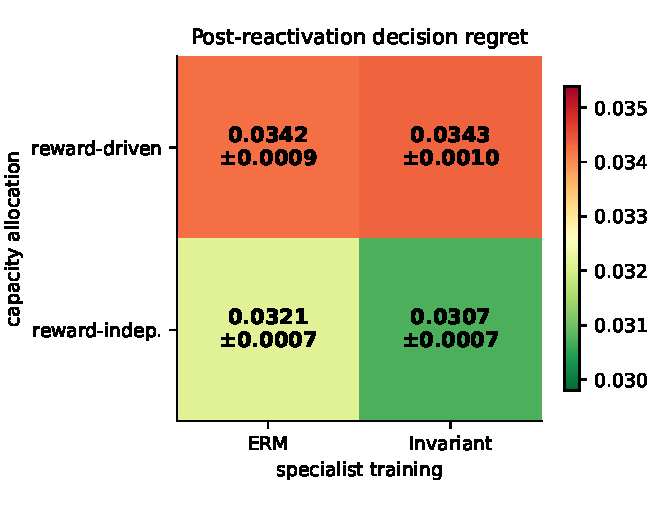
\includegraphics[width=\linewidth]{figures/fig1_2x2.pdf}
        \caption{The $2{\times}2$: the invariance axis is inert in the
        reward-driven row (the predicted asymmetry).}
        \label{fig:2x2}
    \end{subfigure}\hfill
    \begin{subfigure}{0.54\textwidth}
        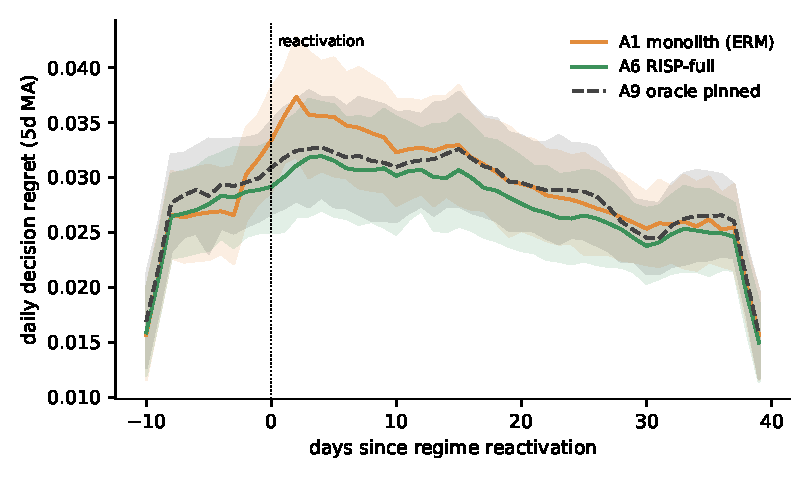
\includegraphics[width=\linewidth]{figures/fig7_trace.pdf}
        \caption{Daily regret aligned on reactivation.}
        \label{fig:trace}
    \end{subfigure}
    \caption{\textbf{Left:} post-reactivation decision regret across
    allocation $\times$ objective (mean $\pm$ 95\% CI, 20 seeds). Cells:
    A1 / A7 (top), A5 / A6 (bottom). \textbf{Right:} mean daily regret
    around reactivations (5-day MA, 95\% CI): the monolith pays a
    relearning transient concentrated in the probe window; \nm{}-full
    tracks the oracle-assignment skyline from day one.}
    \label{fig:headline}
\end{figure}

\begin{figure}[t]
    \centering
    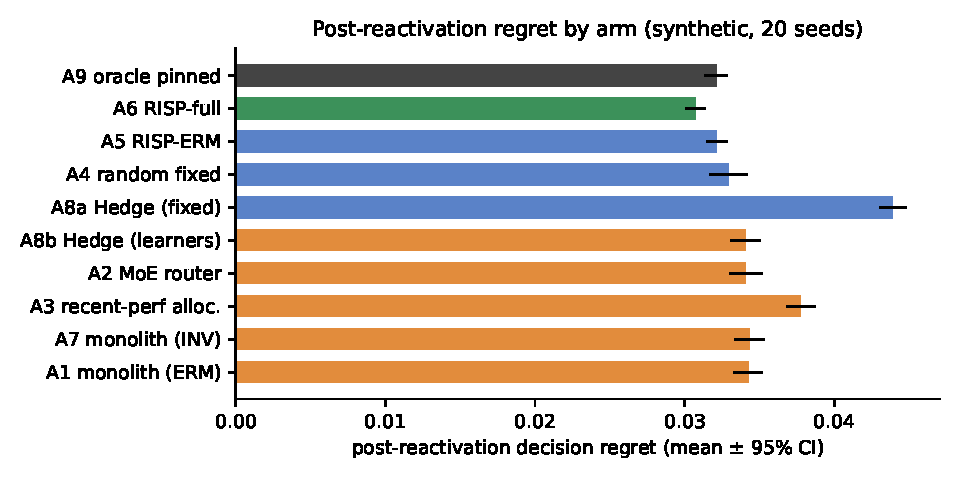
\includegraphics[width=0.86\textwidth]{figures/fig2_arms.pdf}
    \caption{E1, all eleven arms (synthetic, $K{=}2$, hard memory, 20
    seeds). Color encodes class: green = emergent reward-independent +
    invariant; blue = reward-independent (ERM or fixed); orange/red =
    reward-driven; black = oracle skyline. The dissociation separates
    classes, not architectures: every reward-chasing arm clusters with the
    monolith regardless of its machinery.}
    \label{fig:arms}
\end{figure}

Table~\ref{tab:e1} and Figures~\ref{fig:headline}--\ref{fig:arms} give the
headline. Every pre-registered prediction is confirmed
(Holm-corrected Welch tests over 20 seeds):

\textbf{The retention axis is real.} Emergent reward-independent
assignment with identical ERM training cuts post-reactivation regret from
$0.0342$ (A1) to $0.0321$ (A5), $-6.1\%$, $p = 1.3 \times 10^{-3}$ (Holm
$1.0 \times 10^{-2}$). Random fixed niches (A4) sit statistically with A5
($p = 0.28$) but with twice the seed variance---the signature of coverage
gaps: a seed whose random draw covers all four regimes retains like A5; a
seed with an unowned regime pays for it on every reactivation.

\textbf{The invariance axis is real---inside a retaining allocation.}
Holding the emergent assignment fixed, the episode-variance objective cuts
post-reactivation regret from $0.0321$ (A5) to $0.0307$ (A6), $-4.4\%$,
$p = 6.1 \times 10^{-3}$ (Holm $4.3 \times 10^{-2}$). Jointly, A6 improves
on A1 by $10.3\%$ raw ($p = 9.2 \times 10^{-7}$), which is $38\%$ of the
excess over the irreducible noise floor ($0.0342 - 0.0250 = 0.0092$ down
to $0.0057$).

\textbf{The interaction is super-additive, exactly as
Proposition~\ref{prop:additive} predicts.} The invariant objective in a
reward-driven monolith (A7) is indistinguishable from ERM (A7 vs.\ A1
post-reactivation: $p = 0.88$): an objective cannot help a head that was
evicted during dormancy. Per-seed, the interaction index
$I = (\text{A1}{-}\text{A5}) + (\text{A1}{-}\text{A7}) -
(\text{A1}{-}\text{A6}) = -0.0015 \pm 0.0005$ (95\% CI excluding zero):
the joint improvement exceeds the sum of the marginal improvements because
the invariance margin only exists where retention preserves the head it
trained. This asymmetry is the distinctive signature of the two-mechanism
account---a generic ``both tricks help additively'' story would put $I$
at zero, and a shared-cause story would make A7 help. (A7 is directionally
better than A1 \emph{overall}---$0.0266$ vs.\ $0.0269$, not
significant---consistent with the objective helping while heads are alive
and being erased at each eviction.)

\textbf{Reward-driven arms cluster together, as the theory says they
must.} The learned router tracks the monolith ($p = 0.83$); Hedge over
learning experts tracks it too ($0.0341$); the recent-performance
allocator is \emph{worst} among learner arms ($0.0378$)---it not only
forgets dormant regimes but trains specialists on a capital-weighted blend
of foreign regimes throughout, paying interference even in steady state.
The sleeping-experts reading of our problem is answered constructively:
A8a (fixed strategies) retains trivially yet is dominated by every
learning arm everywhere ($0.0439$ post-reactivation, $0.0370$ steady)---
retention without within-niche learning is worth little; A8b (learning
experts) learns but forgets---adaptivity of the \emph{combination} does
not protect the \emph{experts}. The contribution lives exactly in the gap
this pair brackets.

\textbf{\nm{} matches the skyline it was never given.} A6 is
statistically indistinguishable from A10---the hand-pinned oracle
assignment with the same invariant objective ($0.0307$ vs.\ $0.0305$,
$p = 0.72$)---and nominally better than the oracle assignment with ERM
training (A9, $p = 0.011$, marginal after Holm at $0.057$). As in GAUSE,
the value of competition is not beating hand-assignment given the labels
(it cannot); it is \emph{recovering the oracle partition automatically}:
in every seed the population converges to a covering one-per-regime
assignment (the three common regimes pin at affinity $\ge 0.95$; the
rare crisis regime reaches $0.67$--$0.87$---short of the pin threshold
because crisis windows are scarce---but with the correct unique owner
serving throughout, an honest wrinkle we report rather than hide).

\subsection{E0 --- the structure diagnostic on real data, and an honest
null}
\label{sec:e0}

Before any regime-aware mechanism is credited on real data, the
diagnostic-first protocol requires evidence that regime structure
\emph{exists on the decision metric}: an oracle regime-conditioned
predictor (one ridge model per causal regime label, walk-forward refit)
must beat the same machinery under block-shuffled labels. GAUSE's oracle
audit found crypto and commodities carry no exploitable regime structure
under the \emph{prediction} metric \citep{li2026gause}; since
prediction-optimal and decision-optimal differ (the core
predict-then-optimize lesson), we pre-registered the re-test under
decision regret as a finding either way.

\begin{table}[t]
\centering
\small
\caption{E0: structure diagnostic on the decision-regret metric
(walk-forward, second-half evaluation; shuffled = block-label permutation,
10 draws). Negative gap = conditioning is (insignificantly) \emph{worse}
than shuffled. No domain--labeler pair passes; the real-data dissociation
is therefore predicted null, and is (Section~\ref{sec:e1s}).}
\label{tab:e0}
\begin{tabular}{llcccc}
\toprule
\textbf{Domain} & \textbf{Labeler} & \textbf{Real} & \textbf{Shuffled} &
\textbf{Gap} & \textbf{$z$} \\
\midrule
Crypto (5 pairs, daily)      & L1 vol$\times$trend & $0.01220$ & $0.01202$ & $-1.5\%$ & $-0.66$ \\
Crypto (5 pairs, daily)      & L2 filtered HMM     & $0.01212$ & $0.01204$ & $-0.7\%$ & $-0.17$ \\
Commodities (3, daily)       & L1 vol$\times$trend & $0.00834$ & $0.00832$ & $-0.3\%$ & $-0.14$ \\
Commodities (3, daily)       & L2 filtered HMM     & $0.00836$ & $0.00838$ & $+0.2\%$ & $+0.16$ \\
\bottomrule
\end{tabular}
\end{table}

The answer (Table~\ref{tab:e0}) is unambiguous: \textbf{no exploitable
regime structure on the decision metric} in either domain, under either
causal labeler---regime-conditioned regret is statistically identical to
block-shuffled-label regret (all $|z| < 0.7$), and both are identical to a
pooled unconditioned model. The prediction-metric null of GAUSE
\emph{extends} to the decision metric here: the PnO distinction, which in
principle could resurrect structure invisible to prediction error, does
not do so on these panels. We bound the claim honestly: these are small
universes (five crypto pairs, three commodities) at daily frequency with a
standard momentum/volatility feature inventory and two labelers; richer
features, intraday horizons, or larger cross-sections could yet pass the
gate. What the protocol forbids is claiming the mechanism's benefits where
the gate fails---which is exactly what a less guarded evaluation would
have produced, since the machinery happily trains and ``specializes''
on structureless labels (the GAUSE negative control: organization is not
structure).

\subsection{E1s --- the real-data dissociation is null, as the failed gate
predicts}
\label{sec:e1s}

We ran the full eleven-arm comparison on \emph{regime-stitched} real
crypto data: contiguous same-label day-blocks of the actual cross-sections
(real returns, real features), re-arranged into controlled schedules with
the rare regime dormant $\approx 200$ days (20 seeds). All learner arms
are statistically indistinguishable (post-reactivation regret
$0.0134$--$0.0141$; every pairwise $p > 0.2$). Under a failed E0 gate
this is the \emph{predicted} outcome---there is no per-regime structure
for a specialist to retain, so retention cannot pay---and we present it as
the protocol working, not as the mechanism failing: the same arms, the
same code, and the same statistics that produce the sharp dissociation of
Table~\ref{tab:e1} produce a flat table when the precondition is absent.
A method whose evaluation cannot go flat on structureless data should not
be trusted when it goes sharp. (Fallback F1 of the pre-registered design:
where the gate fails on all available real domains, the headline is the
controlled study plus the diagnostic protocol; the equities panel, with
its richer episode inventory, is the planned real-data test.)

\subsection{E2 --- capacity sweep: when does the dissociation close?}
\label{sec:e2}

\begin{figure}[t]
    \centering
    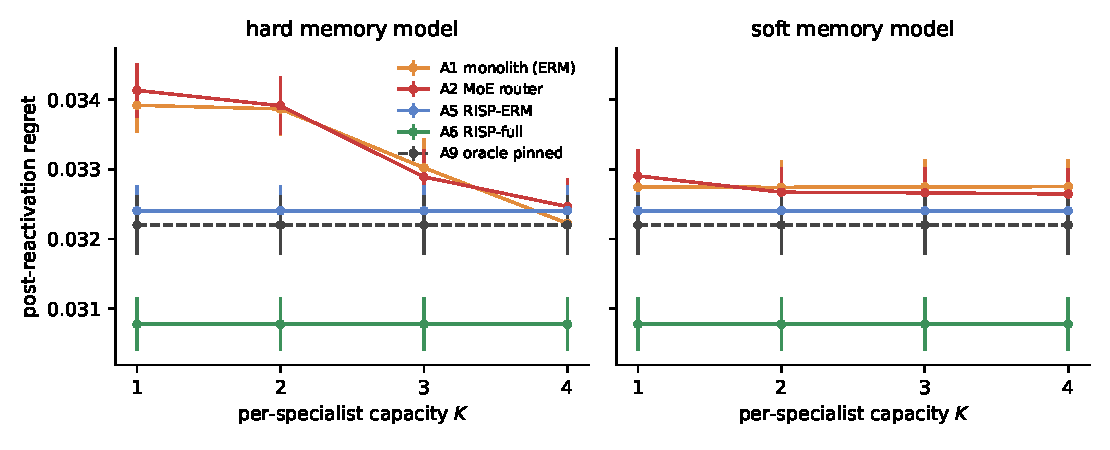
\includegraphics[width=0.95\textwidth]{figures/fig3_capacity.pdf}
    \caption{E2: post-reactivation regret vs.\ per-specialist capacity $K$
    ($R = 4$; 20 seeds; left: hard LRU, right: soft interference).
    Reward-independent arms are flat in $K$; reward-driven arms close the
    gap only as $K \to R$ under hard slots, and never fully close it under
    interference.}
    \label{fig:capacity}
\end{figure}

Sweeping per-specialist capacity $K = 1, \dots, 4$ ($= R$) under both
memory models (Figure~\ref{fig:capacity}): \nm{} arms are \emph{flat in
$K$} (A6: $0.0307$ at every $K$; A5: $0.0321$)---a converged one-per-regime
assignment needs one slot per specialist, and extra capacity is simply
unused. Under the hard model the reward-driven arms improve monotonically
with $K$ and approach the retaining class only at $K = R$ (monolith:
$0.0343 \to 0.0322$, matching A5 at $K{=}4$; router likewise), where
eviction becomes unnecessary and the allocation question dissolves. The
soft (interference) model inverts the diagnosis instructively: with no
eviction, capacity slots stop binding and the reward-driven arms are
\emph{flat} in $K$ at $\approx 0.0328$---gentler than hard eviction at
tight capacity ($0.0343$ at $K \le 2$) but never closing the gap to A6
($0.0307$) at \emph{any} capacity, because graded interference from
foreign updates erodes dormant heads no matter how many slots exist.
Slack capacity is thus one audited boundary of the contribution, with a
caveat that depends on the memory physics: with $K \ge R$ \emph{and}
hard isolation, conditioning alone suffices (the
regime-switching-finance baseline is vindicated exactly there); with
shared representations (the realistic reading for parametric models),
interference keeps the population's structural protection valuable at
every capacity.

\subsection{E3 --- dormancy sweep and the break-even window}
\label{sec:e3}

\begin{figure}[t]
    \centering
    \begin{subfigure}{0.49\textwidth}
        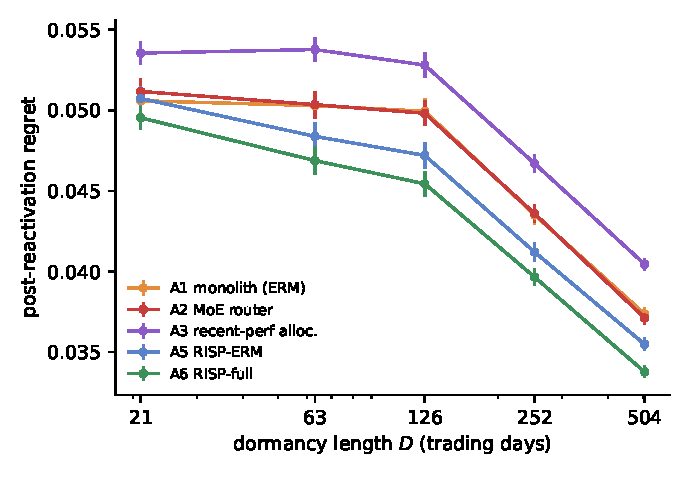
\includegraphics[width=\linewidth]{figures/fig4_dormancy.pdf}
        \caption{Dormancy sweep (E3).}
        \label{fig:dormancy}
    \end{subfigure}\hfill
    \begin{subfigure}{0.49\textwidth}
        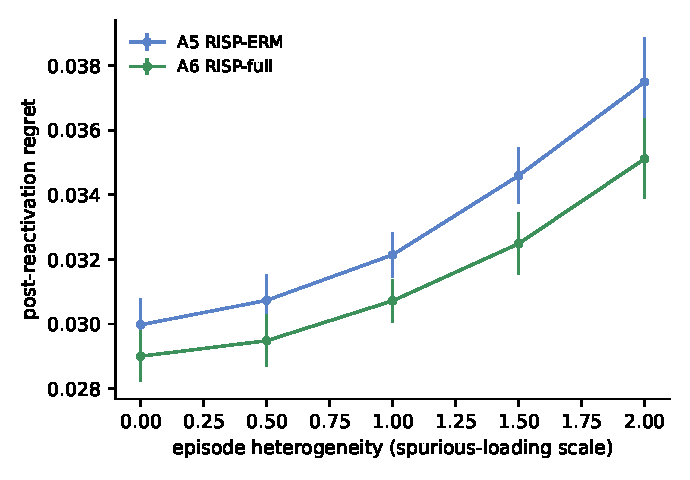
\includegraphics[width=\linewidth]{figures/fig5_heterogeneity.pdf}
        \caption{Episode-heterogeneity sweep (E4).}
        \label{fig:het}
    \end{subfigure}
    \caption{\textbf{(a)} Post-reactivation regret vs.\ dormancy $D$ of the
    focal regime: the reward-driven arms' deficit saturates once $D$
    exceeds the eviction scale (Lemma~\ref{lem:eviction}); levels are not
    comparable across $D$ (schedules differ), arm gaps within each $D$
    are. \textbf{(b)} Fixing the retaining allocation and sweeping episode
    heterogeneity isolates the invariance axis: the ERM$-$INV gap grows
    $2.4\times$ across the sweep.}
    \label{fig:e3e4}
\end{figure}

Controlled schedules place the focal regime's reactivations after dormancy
$D \in \{21, 63, 126, 252, 504\}$ days (Figure~\ref{fig:dormancy}). The
retention gap (A1 $-$ A6 post-reactivation) grows from $0.0015$ at
$D = 21$ to $0.0038$--$0.0044$ for $D \ge 63$ and saturates---the
signature of Lemma~\ref{lem:eviction}: once dormancy exceeds the eviction
scale ($\approx K$ foreign-regime acquisitions, here a few dozen days),
the monolith's head is gone with probability $\approx 1$ and longer
dormancy adds no further loss, while the \nm{} owner's deficit is flat at
zero by construction. The recent-performance allocator degrades fastest
(its capital floor keeps eroding the dormant specialist throughout).
Feeding the measured quantities into Proposition~\ref{prop:breakeven}
(relearning cost $C_{\mathrm{relearn}} \approx 0.004$ per probe day over
$N_p = 15$ days): at a carrying cost of $1\%$ of the per-day probe saving
per idle-specialist-day, retention pays for $D$ between roughly $40$ and
$6{,}000$ days; at $10\%$ carrying cost the window shrinks to
$D \in [\approx 60, \approx 600]$ days---and at carrying costs above
$\approx 15\%$ of the probe saving, \emph{no} dormancy length pays. The
existence of the \emph{upper} break-even is the practically honest point:
idle desks are not free, and a fund whose crisis playbook reactivates
once a decade may rationally let it decay if maintaining it costs enough.

\subsection{E4 --- episode heterogeneity isolates the invariance axis}
\label{sec:e4}

Holding the allocation fixed (emergent, retaining) and sweeping the
episode-heterogeneity scale (the spurious loading's standard deviation
relative to invariant signal) from $0$ to $2\times$ baseline
(Figure~\ref{fig:het}): the ERM specialist degrades steadily
($0.0300 \to 0.0375$ post-reactivation) while the invariant specialist
degrades about $23\%$ slower ($0.0290 \to 0.0351$), so the A5$-$A6 gap
widens monotonically from $0.0010$ to $0.0024$ ($2.4\times$)---the regime-indexed analogue
of the Inv-PnCO heterogeneity result, and direct evidence that the
invariance margin is purchased against episode variability specifically
(at zero heterogeneity the objectives nearly coincide; the small residual
gap is the variance penalty acting as a regularizer against the sixteen
distractor features). Reactivation is an out-of-distribution event
\emph{within} one's own regime to precisely the degree that episodes
differ; retention solves dormancy, and this axis is what remains after.

\subsection{E5 --- ablations}
\label{sec:e5}

\begin{figure}[t]
    \centering
    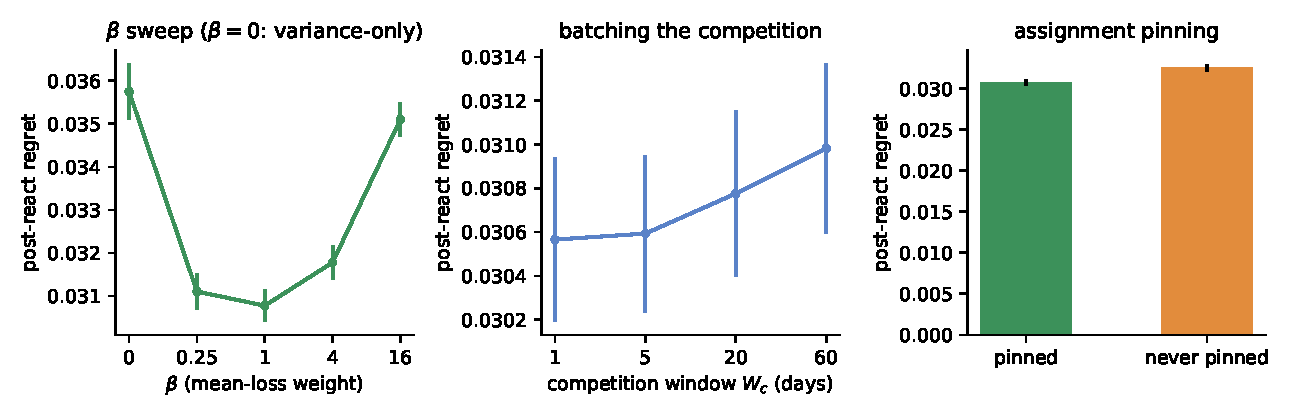
\includegraphics[width=0.98\textwidth]{figures/fig8_ablations.pdf}
    \caption{E5 ablations (post-reactivation regret, 20 seeds).
    \textbf{Left:} the invariance objective is U-shaped in $\beta$ and the
    variance-only control ($\beta = 0$) fails below retained ERM.
    \textbf{Center:} robustness to the competition window $W_c$ (the
    revised batching prediction, Remark~\ref{rem:batching}).
    \textbf{Right:} pinning the converged assignment matters.}
    \label{fig:ablations}
\end{figure}

\textbf{$\beta$ sweep, and the variance-only control fails as predicted.}
Post-reactivation regret is U-shaped in the mean-loss weight:
$\beta = 0$ (variance only) gives $0.0356$---\emph{worse than retained
ERM} ($0.0321$)---confirming in the decision setting the Inv-PnCO
finding that the variance term alone is degenerate (a head can achieve
zero episode-variance by being uniformly bad); the plateau
$\beta \in [0.25, 4]$ gives $0.0307$--$0.0317$; very large $\beta = 16$
degrades to $0.0352$---worse than the retained-ERM arm itself
($0.0321$), which is the honest reading: $\beta$ multiplies the
effective gradient magnitude, so $\beta = 16$ is not ``clean ERM
recovered'' but an unstably large step on the mean term (A5 remains the
correct $\beta \to \infty$ reference, trained at the proper rate). The
objective needs both terms, and is insensitive to $\beta$ across an
order of magnitude.

\textbf{Competition-window sweep.} $W_c \in \{1, 5, 20, 60\}$ days yields
$0.0303$, $0.0306$, $0.0307$, $0.0309$: flat, with per-step competition
marginally \emph{best}---the revision of our pre-registered batching
expectation discussed in Remark~\ref{rem:batching}. The mechanism's
robustness to its main scheduling hyperparameter is itself a deployment
asset.

\textbf{Niche bonus and pinning.} Competition alone ($\lambda = 0$)
reaches $0.0314$ versus $0.0307$ with the default shaping
($\lambda = 0.3$)---the bonus accelerates but does not cause the
assignment, consistent with GAUSE's $\lambda$ ablation. Disabling pinning
costs $0.0320$ versus $0.0307$: keeping competition perpetually open
re-admits exactly the reward-coupling the mechanism exists to remove,
though the EG dynamics' inertia limits the damage.

\subsection{E6 --- audit: when retention is worthless}
\label{sec:e6}

\begin{figure}[t]
    \centering
    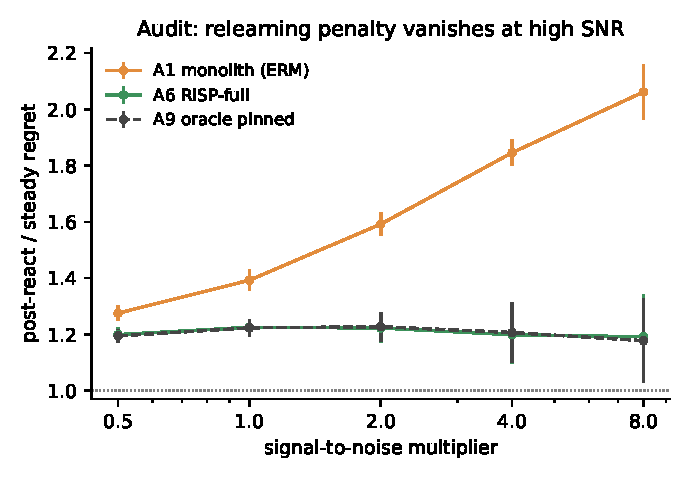
\includegraphics[width=0.55\textwidth]{figures/fig6_snr_audit.pdf}
    \caption{E6 audit: the relearning penalty (post-reactivation regret
    relative to own steady state) as the signal-to-noise multiplier
    sweeps $0.5\times$--$8\times$. The monolith's relative penalty grows,
    but its absolute steady level collapses; the \nm{} advantage inverts
    near $2$--$3\times$ (see text).}
    \label{fig:snr}
\end{figure}

This experiment exists because our first implementation refuted us. At the
default parameters of an early prototype (signal-to-noise an order of
magnitude above realistic daily cross-sections), \emph{no arm separated
from any other}: the monolith relearned an evicted regime within two to
five days, the probe window scored mostly converged behavior, and
retention was demonstrably worthless. Rather than discard the parameter
regime, we promoted it to an audit axis. Sweeping the signal-to-noise
multiplier over $\{0.5, 1, 2, 4, 8\}$ (Figure~\ref{fig:snr}):

\begin{itemize}
    \item The monolith's relearning penalty (post-reactivation over steady
    regret) grows from $1.28\times$ to $2.06\times$ with SNR---relative
    relearning cost rises---but its \emph{absolute} steady level collapses
    ($0.0296 \to 0.0159$), because strong signal is refit almost
    instantly and then exploited deeply.
    \item The \nm{} advantage over the monolith is $+8.3\%$ at
    $0.5\times$, $+10.3\%$ at baseline, $+7.0\%$ at $2\times$---then
    \emph{inverts}: $-13.1\%$ at $4\times$ and $-49.3\%$ at $8\times$. At
    high SNR the episode-specific loading is itself strongly exploitable,
    and an ERM monolith that greedily refits each episode beats an
    invariant specialist that on principle refuses to chase it. The
    skyline arm inverts identically (A9 tracks A6), confirming this is a
    property of the \emph{regime}, not of our assignment mechanism.
\end{itemize}

The audit therefore draws the mechanism's boundary as a measured
crossover, near $2$--$3\times$ our baseline calibration: \nm{} pays where
signals are weak enough that relearning is slow and episode-chasing does
not compensate---which is the empirically realistic regime for daily
cross-sectional return prediction---and is counterproductive where
within-episode signal is strong, fast to fit, and worth chasing. This is
the decision-domain analogue of GAUSE's stale-specialist result under
intra-regime drift: reward-independent retention is an asset under
dormancy and a liability under exploitable drift, and the honest
deliverable is the location of the boundary.

\subsection{Statistical protocol and what we deliberately do not claim}
\label{sec:stats}

All headline comparisons are Welch tests over 20 independent seeds with
Holm--Bonferroni correction within each experiment's pre-registered pair
family; tables report mean $\pm$ 95\% CI. The synthetic and stitched
experiments expose every arm to identical data streams per seed (paired
design). We do \emph{not} report Sharpe ratios, deflated or otherwise, for
the synthetic headline---regret against a known optimum is strictly more
informative when ground truth exists---and we make no claim of live
trading profitability anywhere: by the E0 gate, the panels where we could
have manufactured such claims do not carry the structure that would make
them meaningful. For any future real-data deployment passing the gate, the
protocol of record is: deflated Sharpe \citep{bailey2014deflated} for any
P\&L claim, an SPA/Reality-Check test \citep{hansen2005spa, white2000reality}
across the arm family, transaction costs at $5/10/25$ bps with borrow,
nested walk-forward for every hyperparameter, and the
break-even-dormancy carrying-cost analysis of
Proposition~\ref{prop:breakeven}---pre-committed here.

\subsection{Synthesis}

Across E0--E6 the two-axis account survives every test we could construct
against it, and fails exactly where it claims it should fail. Retention is
an allocation property: every reward-independent covering arm retains
(A4--A6, A9, A10), every reward-chasing arm relearns (A1--A3, A8b), the
boundary is crisp ($p \sim 10^{-6}$ for the class separation), and no
training objective crosses it (A7). Invariance is an objective property:
it pays only inside a retaining allocation (super-additive interaction,
CI excluding zero), grows with episode heterogeneity (E4), and requires
both of its terms ($\beta$ sweep). The mechanism needs its preconditions:
bounded capacity (E2), real dormancy (E3), weak-signal relearning (E6),
and verifiable regime structure (E0/E1s)---each audited with the
experiment that locates its boundary. Where all preconditions held, the
emergent system matched the hand-designed skyline without being given the
assignment; where any failed, the system honestly bought nothing.

%=============================================================================
\section{Discussion}
%=============================================================================

\paragraph{Why two mechanisms, not one.} The temptation in both
literatures is monism. Continual-learning work treats non-stationarity as
forgetting and reaches for retention; OOD-generalization work treats it as
shift and reaches for invariance. The financial setting forces the
synthesis because its non-stationarity is genuinely two-layered: regimes
\emph{recur} (so there is something worth retaining) and recurrences
\emph{differ} (so retention alone retains the wrong thing). The
super-additive interaction is the empirical signature that the layers are
real: each mechanism's value is contingent on the other having done its
job. We conjecture this structure---retain the niche, generalize within
it---is generic to any domain with recurring-but-drifting modes: climate
regimes, epidemic waves, demand seasons, adversary playbooks.

\paragraph{The allocator, not the org chart.} Multi-strategy funds already
silo desks by regime---the practitioner instantiation of
reward-independent assignment. \nm{}'s contribution to that practice is
not the silo but the analysis of what destroys it: recent-performance
capital allocation \emph{across} silos (our A3, the industry's default)
erodes dormant desks at a rate set by its capital floor, and a learned
router---the modern ML upgrade---fails identically and for the same
structural reason (Proposition~\ref{prop:dichotomy}). The emergent
mechanism additionally shows the silo map need not be designed: at
$N \gtrsim R$ it is recovered automatically, matching the hand-pinned
skyline, with graceful degradation documented when competition's
preconditions weaken (the unpinned crisis niche of Section~\ref{sec:e1}).

\paragraph{What the diagnostic-first protocol buys.} The most consequential
result in this paper for applied work is arguably the null: two real asset
classes, two causal labelers, and a decision-metric oracle test that
refuses to certify regime structure---after which the full eleven-arm
machine, run anyway, produces exactly the flat table the refusal predicts.
The protocol converts ``our regime-aware method beat baselines on a
backtest'' (unfalsifiable in the presence of label noise and selection)
into two separable, individually falsifiable claims: \emph{structure
exists here} (E0, cheap, runs before any method) and \emph{given
structure, the mechanism captures it} (E1, controlled). We commend the
split to the regime-aware finance literature at large.

%=============================================================================
\section{Limitations}
\label{sec:limitations}
%=============================================================================

\begin{enumerate}
    \item \textbf{The headline is synthetic; the real-data result is a
    null.} Our dissociation is demonstrated where its preconditions
    verifiably hold---controlled markets with known regime structure,
    episode heterogeneity, and realistic SNR---because on the real panels
    available to us the E0 gate fails and the dissociation is
    (correctly) absent. We regard gate-then-claim as the right
    epistemics, but the constructive real-data demonstration remains
    undone: the planned equities panel (S\&P~500 constituents, 1990--2025,
    with 2000/2008/2011/2015/2018/2020/2022 as crisis episodes), richer
    feature inventories, and intraday horizons are the concrete next
    test, and the protocol pre-commits its statistics
    (Section~\ref{sec:stats}).
    \item \textbf{Small real universes.} Five crypto pairs and three
    commodities at daily frequency; the E0 null is bounded to these
    panels, these labelers (L1/L2), and this feature inventory. A failed
    gate on richer data would be informative; a passed gate would
    activate the E1 protocol on real data. Neither has been run.
    \item \textbf{Assumption~\ref{ass:hyper} idealizes episodes.} Real
    episodes are neither independent (macro memory links crises) nor
    exchangeable (secular drift in market microstructure), and crisis
    regimes offer 5--7 episodes at best---the $O(B/\sqrt{E_r})$
    estimation terms in Lemma~\ref{lem:transfer} are not decorative. The
    sub-episode and cross-asset mitigations of Section~\ref{sec:mechanism}
    enlarge the environment set but introduce their own dependence; we
    flag both rather than resolve them.
    \item \textbf{Theory register.} Propositions~\ref{prop:dichotomy}--%
    \ref{prop:additive} are idealized-model results: the reward-driven
    eviction rate assumes per-step foreign-update probability $p > 0$
    (verified by construction in our arms, plausible but unverified for
    arbitrary allocators), and we claim no adversarial-regret guarantee
    for the coupled winner-take-all dynamics. The bound's additivity
    motivates but does not entail the empirical super-additivity; we
    measure the latter.
    \item \textbf{The mechanism inverts under strong exploitable drift.}
    E6 is a limitation stated as an experiment: at high within-regime SNR,
    invariant retention loses to episode-chasing ERM by up to $49\%$. Any
    deployment must locate itself on the E6 axis first; a staleness
    trigger in the GAUSE style (re-opening competition on confident
    underperformance) is the known remedy and is future work here.
    \item \textbf{Capacity as a binding constraint is a modeling choice.}
    As in GAUSE, a purely tabular learner could hold all regimes; the
    contribution is conditional on capacity binding (true for fixed-size
    parametric models and for the operational reading---calibration
    attention, infrastructure---of strategy pools). The soft-interference
    results (E2) show the dissociation does not depend on the discrete
    eviction model.
    \item \textbf{Task-incremental scope.} Every arm receives the same
    causal regime label; the comparison is information-symmetric, but
    inferring regimes while specializing (class-incremental) is unsolved
    here. GAUSE's label-free variant collapsed under real feature overlap,
    and we expect the financial case to be at least as hard; we do not
    claim otherwise.
\end{enumerate}

%=============================================================================
\section{Conclusion}
%=============================================================================

We decomposed non-stationary financial decision error into two
independently controlled failure modes---between-regime forgetting, owned
by the capacity allocator, and within-regime drift, owned by the training
objective---and showed theoretically and experimentally that fixing either
without the other forfeits most of the available improvement, while
fixing both recovers the hand-designed skyline without hand design. The
enabling property, imported from GAUSE and ported to decision-focused
learning, is reward-independence of the converged assignment; the new
axis, imported from invariant predict-and-optimize and ported to recurring
regimes, is episode-variance penalization of a decision-focused loss; the
bridge between their guarantee languages is one Pinsker step. Around the
mechanism we built the evaluation standard we believe the area needs:
pre-registered orderings, a structure diagnostic that runs before claims,
audits that locate every boundary of validity, and the discipline of
reporting the predictions the data refused. When the regime returns, the
specialist who kept the playbook---and kept it general---decides best;
this paper says precisely when that sentence is true, and how to check.

\bibliographystyle{plainnat}
\bibliography{references}

\end{document}
